\textbf{{1. UDP校验}}

{{a. }}\textbf{{{UDP校验只提供差错检测}{。}}}

b.
在计算校验和时,要在UDP用户数据报之前临时加上12B的伪首部。{其中,伪首部包括源IP地址字段、目的IP地址字段、全0字段、协议字段(UDP固定为17)、UDP长度字段。}

{\textbf{{注意:}}一定要记住伪首部只用于计算和验证校验和,其既不向下传送,也不向上递交。}

{{\textbf{2. UDP校验的注意事项}}}\\

\textbf{1)}校验的时候若UDP数据报数据部分的长度不是偶数字节,则需要填入一个全0B,如下图所示。但是此字节和伪首部一样,是不发送的。

\textbf{2)}如果UDP校验和校验出UDP数据报是错误的,可以丢弃,也可以交付给上层,但是需要附上错误报告,即告诉上层这是错误的数据报。

\textbf{3)}通过伪首部,不仅可以检查源端口号、目的端口号和UDP用户数据报的数据部分,\textbf{还可以检查IP数据报的源IP地址和目的地址。}

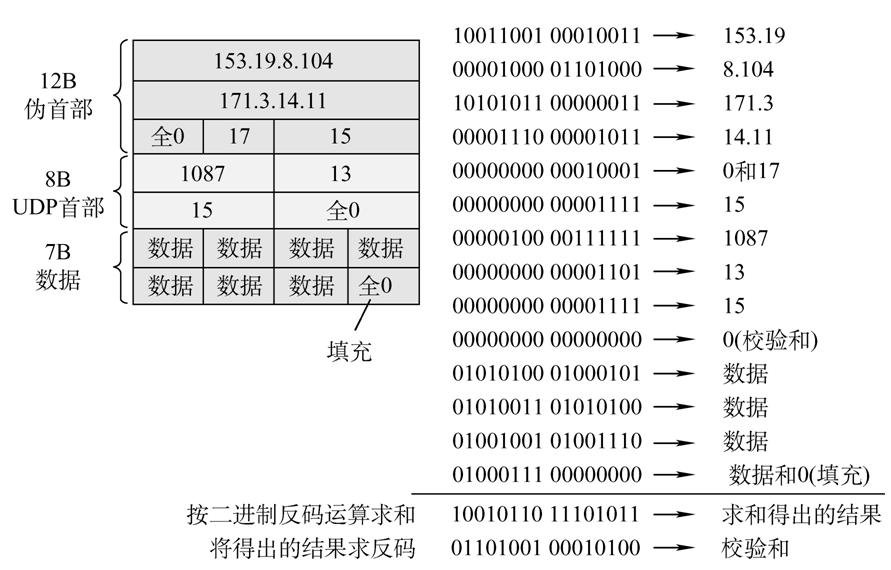
\includegraphics[width=3.33333in,height=2.13542in]{png-jpeg-pics/3D3FDD1E49C063F30606CFD1913A3BBA.png}

按二进制反码计算后,\textbf{当无差错时其结果应该为全1};否则就表明有差错出现,接收方就应该丢弃这个UDP报文。
